\newpage
\section{Systemöversikt}
QuadOpt är uppdelat i flera mindre delsystem, för att vara mer lätthanterligt och lättare att utveckla.

\subsection{Systembeskrivning}
%QuadOpt kommer kunna köras via två olika typer av gränssnitt. Det ena är vårt egetutvecklade GUI och det andra är anrop via Matlab.

%\subsubsection{GUI}
%\subsubsection{Matlab}

\begin{figure}[h]
	\begin{center}
		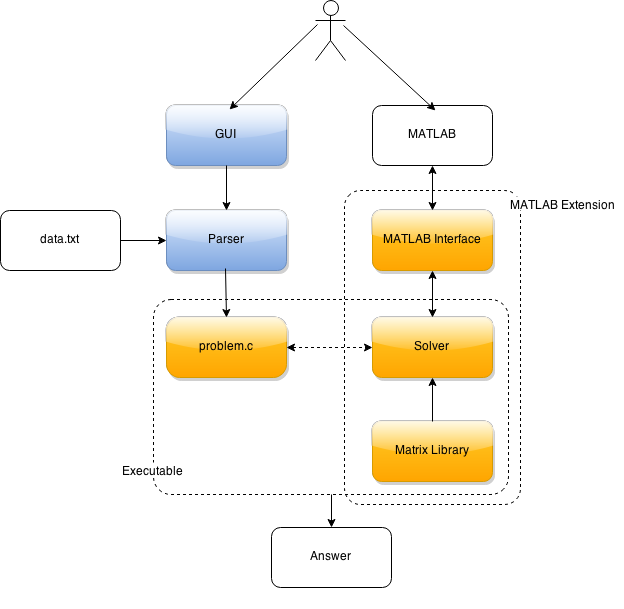
\includegraphics[scale=0.5]{bilder/arkitektur.png}
	\end{center}
	\caption{Arkitektur av systemet.}
\end{figure}

%\subsection{Beräkningar}
%Kommer utföras i lösaren, kommer använda vårt egna matrisbibliotek Matlib för att snabba upp beräkningarna.